
\documentclass[10pt,a4paper]{article}
\usepackage[utf8]{inputenc}
\usepackage[french]{babel}
\usepackage[left=2cm,right=2cm,top=2cm,bottom=2cm]{geometry}
\usepackage{hyperref}
\usepackage{graphicx}

%opening
\title{SECO TP 1}
\author{Nicolas Vadkerti}
\usepackage{listings} % Required for inserting code snippets
\usepackage[usenames,dvipsnames]{color} % Required for specifying custom colors and referring to colors by name

\definecolor{DarkGreen}{rgb}{0.0,0.4,0.0} % Comment color
\definecolor{highlight}{RGB}{255,251,204} % Code highlight color

\lstdefinestyle{Style1}{ % Define a style for your code snippet, multiple definitions can be made if, for example, you wish to insert multiple code snippets using different programming languages into one document
language=Bash, % Detects keywords, comments, strings, functions, etc for the language specified
backgroundcolor=\color{highlight}, % Set the background color for the snippet - useful for highlighting
basicstyle=\footnotesize\ttfamily, % The default font size and style of the code
breakatwhitespace=false, % If true, only allows line breaks at white space
breaklines=true, % Automatic line breaking (prevents code from protruding outside the box)
captionpos=b, % Sets the caption position: b for bottom; t for top
commentstyle=\usefont{T1}{pcr}{m}{sl}\color{DarkGreen}, % Style of comments within the code - dark green courier font
deletekeywords={}, % If you want to delete any keywords from the current language separate them by commas
%escapeinside={\%}, % This allows you to escape to LaTeX using the character in the bracket
firstnumber=1, % Line numbers begin at line 1
frame=single, % Frame around the code box, value can be: none, leftline, topline, bottomline, lines, single, shadowbox
frameround=tttt, % Rounds the corners of the frame for the top left, top right, bottom left and bottom right positions
keywordstyle=\color{Blue}\bf, % Functions are bold and blue
morekeywords={}, % Add any functions no included by default here separated by commas
numbers=left, % Location of line numbers, can take the values of: none, left, right
numbersep=10pt, % Distance of line numbers from the code box
numberstyle=\tiny\color{Gray}, % Style used for line numbers
rulecolor=\color{black}, % Frame border color
showstringspaces=false, % Don't put marks in string spaces
showtabs=false, % Display tabs in the code as lines
stepnumber=5, % The step distance between line numbers, i.e. how often will lines be numbered
stringstyle=\color{Purple}, % Strings are purple
tabsize=2
}

\newcommand{\insertcode}[2]{\begin{itemize}\item[]\lstinputlisting[caption=#2,label=#1,style=Style1]{#1}\end{itemize}} 


% \insertcode{"Scripts/example.pl"}{Nena would be proud.} 

\begin{document}

\maketitle
\url{https://github.com/SlaynPool/CR_SECO/}
\section{Attaques hors ligne}

\subsection{AP HTTP}
On recupere le fichier .ino disponible sur moodle, on modifie les parametres de l'application comme ceci:
\insertcode{code/AP_HTTPHead.ino}{Modification du .ino}
\begin{figure}[h!]
\centering
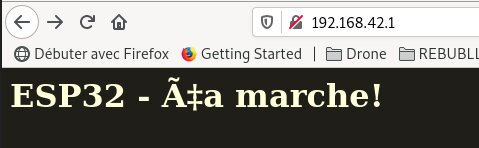
\includegraphics[scale=0.20]{image/1.jpg}
\caption{Premier Page}
\label{fig:net }
\end{figure}

 \begin{figure}[h!]
\centering
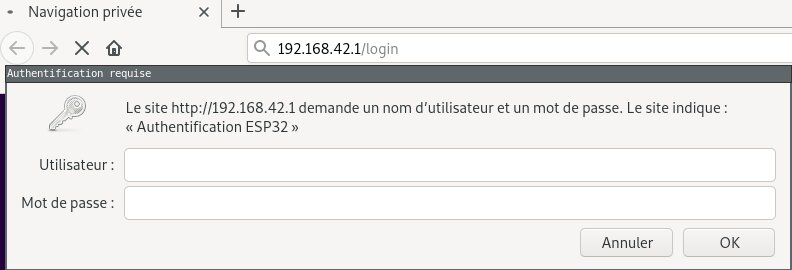
\includegraphics[scale=0.20]{image/2.jpg}
\caption{Connection }
\label{fig:net }
\end{figure}
\begin{figure}[h!]
\centering
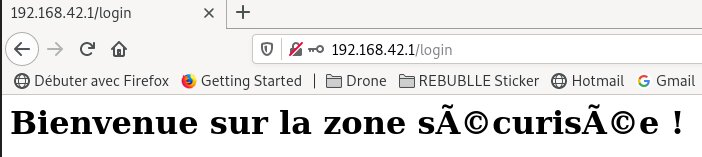
\includegraphics[scale=0.20]{image/3.jpg}
\caption{Reussite }
\label{fig:net }
\end{figure}
\subsection{Fouille du .bin de mon voisin}
Voici la ligne de compilation executer par l'IDE: \\
\insertcode{code/compil.txt}{compilation}

Le fichier .bin est generer dans  tmp arduino build 64730
Buddy ma fourni son binaire qui tourne sur son ESP. Grace à Hexdump nous avons converti le binnaire en caractère lisible:
\insertcode{code/hexcom.txt}{traduction}

 On voit que quand je cherche le mot SSID, il me repond que ce mots existe à la ligne 00001110. Nous regardons donc a cette ligne pour voir si il ya pas des mots de passes à proximité de la déclaration du SSID et :
 \insertcode{code/result.hex}{On a trouvé !}
 On comprend rapidement que le premier mots de passes que l'on semble voir est le mots de passes de l'authentification WEB, notament car ``buddy'' n'est pas le SSID que je vois depuis ma carte Wifi mais plutot ``cestquoilecode''
 Donc on déduis grâce au binaire que on pourra passer l'authentification Web grâce au couple User/PWD : buddy/98765432\\
 Et le Mot de passe du reseau Wifi : 23456789
 
 \subsection{Dump d'un binaire depuis une carte}
 J'ai echangé mon ESP32 avec Buddy. Je m'attend donc à obtenir le même resultat que précedement.\\
 Pour dumper la memoire d'un ESP32, nous allons utiliser la commande suivante :
 \insertcode{code/dump.txt}{Dump de la memoire flash d'un ESP}
 On determine L'OFFSET  grace à cette ligne vu dans l'arduino IDE:
 \insertcode{code/onsaitladdresse.txt}{Compilation}
 Le binaire sera donc ecrit à partir de l'adresse 0x10000 donc on regarde directement à l'adresse 0x10000+0x1110 soit 0x11110 

 \subsection{Remise à Zero de la memoire flash de L'ESP32}
 Pour cela il suffit d'utiliser la commande suivante:
 \insertcode{code/erase.txt}{esptool.py erase flash}
 On voit que la commande a correctement fonctionner car quand nous lisons la memoire de la carte, nous n'avons que des ``ff''
 
 \subsection{L'historique des anciens programmes restes sur L'ESP32}
 
 En Effet, si on compile/téléverse le programes plusieurs fois sur la carte, tous en modifiant le mots de passe de l'AP par exemple( 87654321, 17654321, 27654321), on se rend compte que les anciens MDP sont encore visibles:
 \insertcode{code/oldpPwd.txt}{On voit les anciens PWD}
 On peut donc voir que le Premier MDP est stocké à l'adresse 0x0a540\\
 Le second MDP est stocké à l'adresse 0x0a8e0\\
 Le mots de passe actuelle est stocké à l'adresse 0x0ac80 et l'ancienne adresse 0x011180
 \newpage
 \section{Attaques en fonctionnement à distance}
 \subsection{Creation d'un dictionnaire}
 On veut créer un dictonnaire contenant chaques mdp avec que des chiffres, sans doublons:
 \insertcode{code/genDico/genDico.py}{Mon générateur de dictionnaire}
Le dictionnaire généré semble etre de la taille que vous nous avez indiquez et semble générer les bons nombres
\insertcode{code/genDico/taille.txt}{Mon dictionnaire}\newpage
\subsection{Utilisation de aircrack-ng sur le fichier ap1.pcap}
On utilise aircrack-ng comme ceci :
\insertcode{code/aircrack.txt}{aircrack}
Nous avons donc reussi à obtenir la clé de l'AP et celle-ci est ``54921037`` !!!!
\subsection{Décodage de trame http}
Nous avons trouvé la clé du reseau précedament, il faut donc que WireShark la connaisse pour pouvoir déchiffré les trames:
\begin{figure}[h!]
\centering
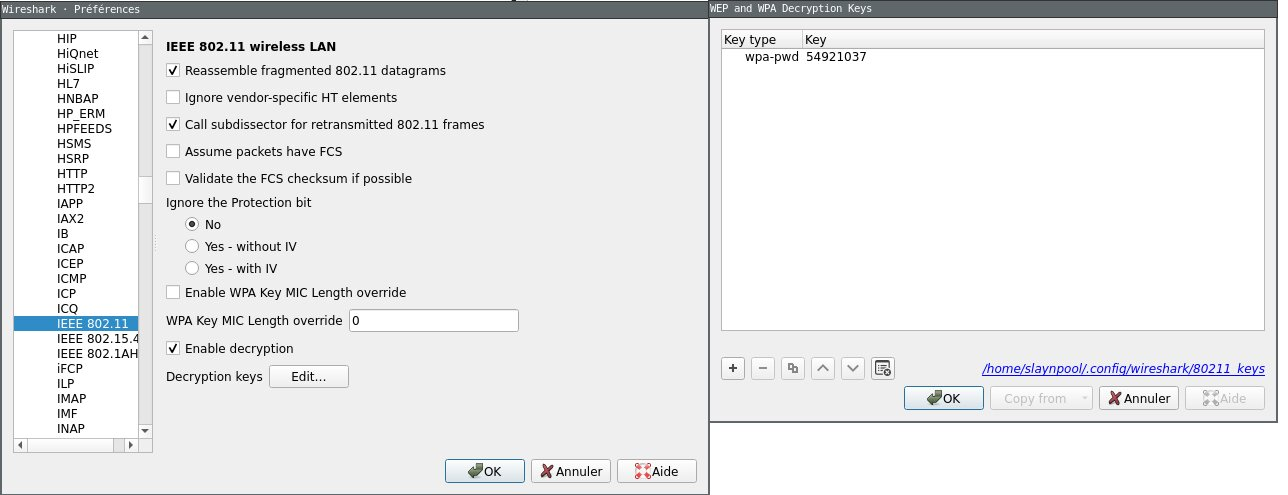
\includegraphics[scale=0.30]{image/5.jpg}
\caption{Ajoute de la Clé dans wireshark}
\label{fig:net }
\end{figure}
A partir de là, nous somme donc capable d'interpréter les trames et donc les trames http :
On choisis une trame GET/login:
\begin{figure}[h!]
\centering
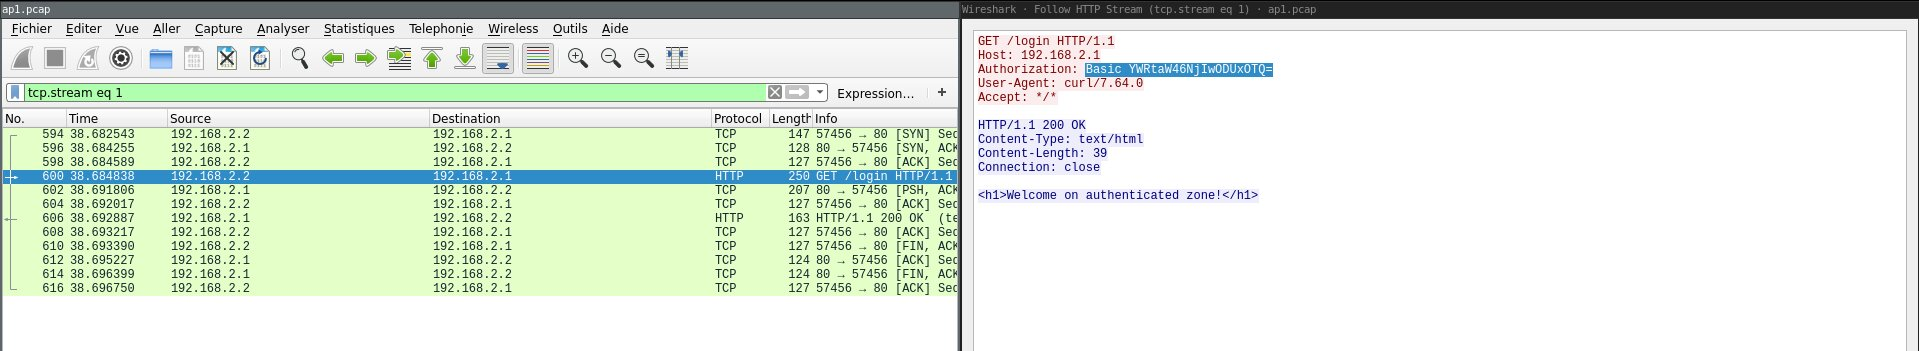
\includegraphics[scale=0.250]{image/4.jpg}
\caption{Ajoute de la Clé dans wireshark}
\label{fig:net }
\end{figure}
\\
Donc on sait que c'est du base64\\
\insertcode{code/base64.txt}{Decodage du base 64}
Le couple USER/PWD est admin/62085194

\subsection{Realisation de la manip sur la puce de mon voisin}
Tout d'abord, on veut savoir quelle channel utilise notre voisin. Son reseau s'appelle ''cestquoilecode``.
\insertcode{code/ChannelWant}{Determination de la bande de son voisin}
On configure donc notre carte sur le chanel 5 et on passe en mode monitor.
\insertcode{code/confWifi}{Configuration de la carte wifi}
J'ai donc fais une capture de trame en demandant à Buddy de se connecter à l'AP, pour qu'il génére le HandShake et qu'il soit visibles dans ma capture. Le problème à etait que je n'ai pas vu le handshake complet. J'ai donc changé de carte Wifi et fais et bien récupérer le HandShake, lancé AirCrack-ng et Bingo :

\insertcode{code/manipBuddy}{On à reussi}
On indique donc maintenant à Wireshark la clé pour qu'il puisse décrypter les trames.
NOTE IMPORTANTE: Pour pouvoir décrypter les trames HTTP, on doit avoir l'intergalité de la connection, CàD, le HandShake, et les trames HTTP.
\begin{figure}[h!]
\centering
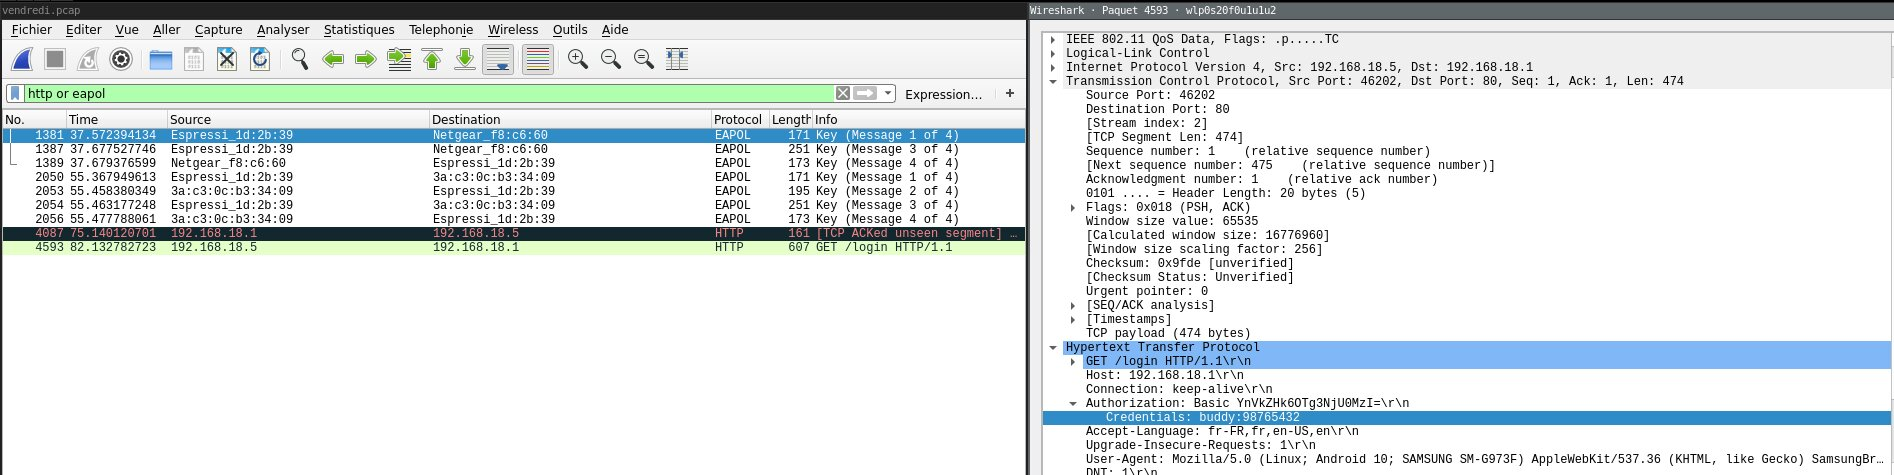
\includegraphics[scale=0.250]{image/6.jpg}
\caption{On a trouvé l'identification HTTP}
\label{fig:net }
\end{figure}
\newpage
\subsection{Verification de la validité d'un couple USER/PWD}
En ce basant sur le cours et la page Wikipedia fourni, voici mon ''programe``:
\insertcode{manip/digest_auth.sh}{Digest Auth }
\subsection{Détérmination du mots de passe de l'utilisateur dans le fichier ap2.pcap}
Tous d'abord, on doit trouver le mots de passes de l'AP :
\insertcode{code/manipAP2I}{71862093}
On peut ainsi récuperer les informations de connactions dans la trame de connection:
\begin{figure}[h!]
\centering
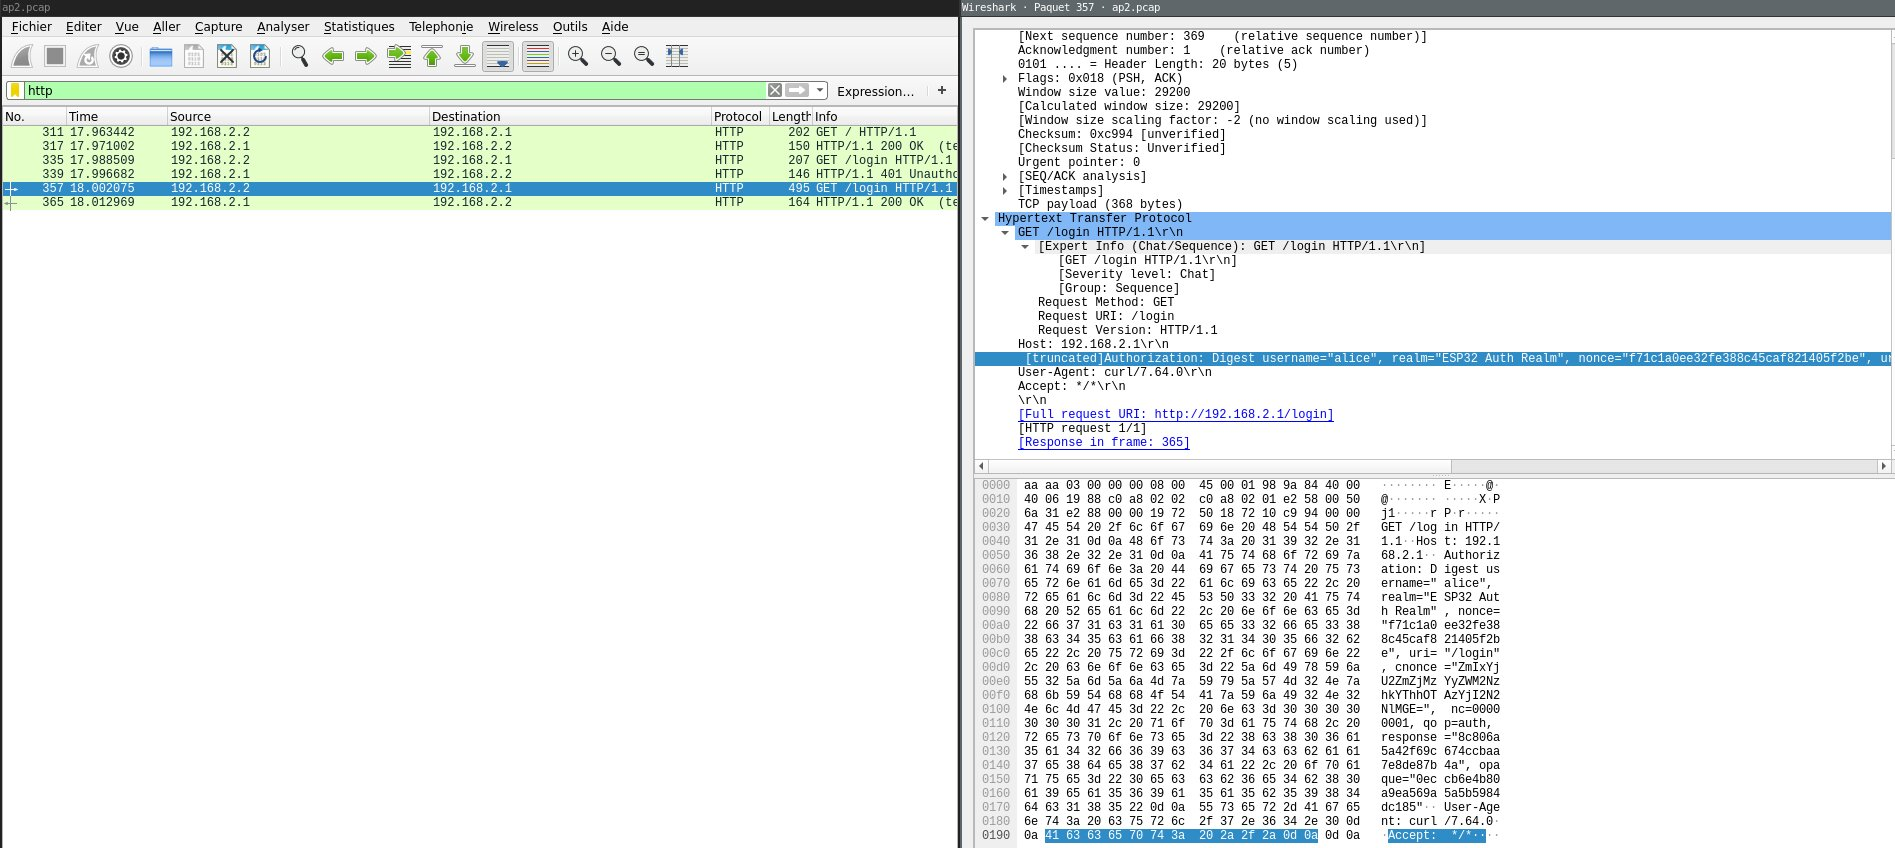
\includegraphics[scale=0.250]{image/7.jpg}
\caption{Ajoute de la Clé dans wireshark}
\label{fig:net }
\end{figure}
Nous avons donc toutes les informations pour brute Force le mot de passe. Nous allons utiliser le meme code qui vérifier la validité du mot de passe réecrie en Python pour des raisons de rapidités:
\insertcode{manip/digest_authAP2.py}{digest authentification python}
\newpage
\subsection{Reproduction sur une vrai puce en fonctionnement}
Donc on determine le channel de la puce et on configure notre carte wifi en mode monitor sur le bon channel:
\insertcode{code/puce/1}{Setup}
On fait une capture de trame pendant une connexion à l'AP et au site sécuriser, au moins nous n'aurons pas à refaire de capture de trame:
\begin{figure}[h!]
\centering
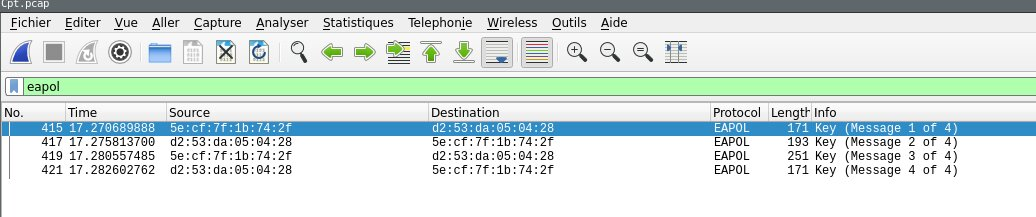
\includegraphics[scale=0.500]{image/8.jpg}
\caption{Capture}
\label{fig:net }
\end{figure}
On utilise AirCrack-ng:
\insertcode{code/puce/2}{AirCrack}
On décrypte les trames avec wireshark :
\begin{figure}[h!]
\centering
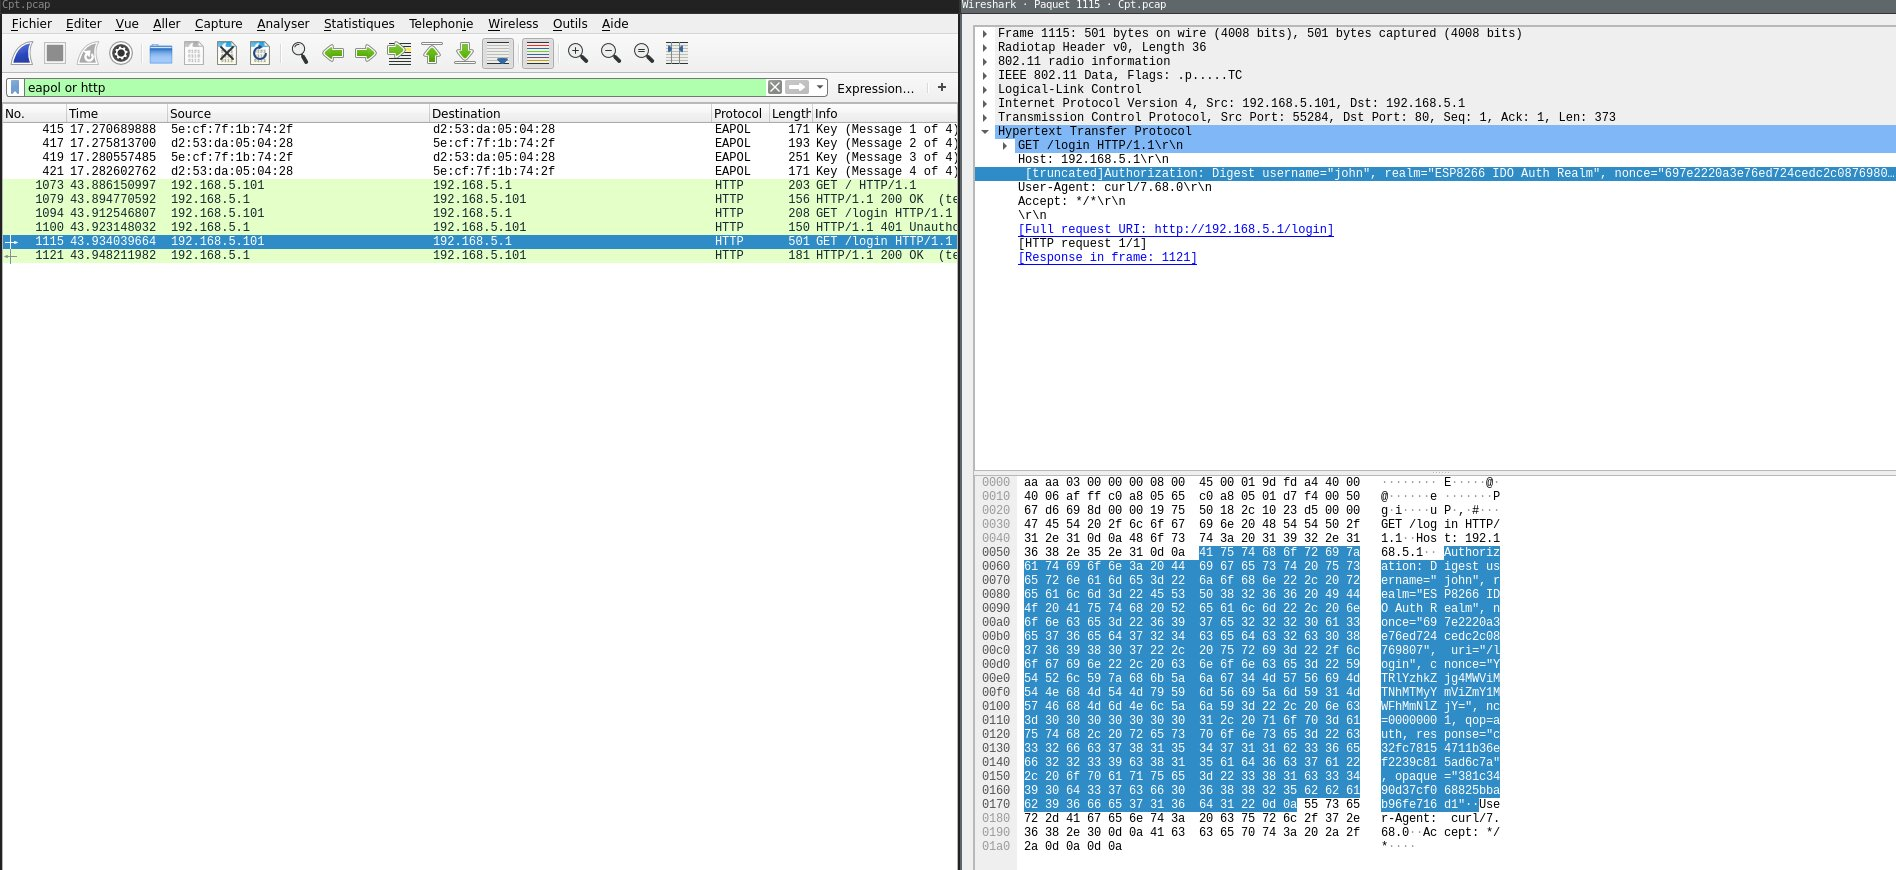
\includegraphics[scale=0.250]{image/9.jpg}
\caption{Trame HTTP}
\label{fig:net }
\end{figure}
On Brute force avec mon programme python en modifiant les variables par celle trouvé dans la capture:
\insertcode{manip/puce/digest_authAP2.py}{Le code est 65983241}
Donc, nous savons à present que le mot de passe nessacaire pour ce connecter à l'AP est : 61495327\\
Le nom d'utilisateur est : john (On le sais grace à la trame HTTP)\\
Et que le mot de passe de john est : 65983241 

On peut donc ce connecter :
\begin{figure}[h!]
\centering
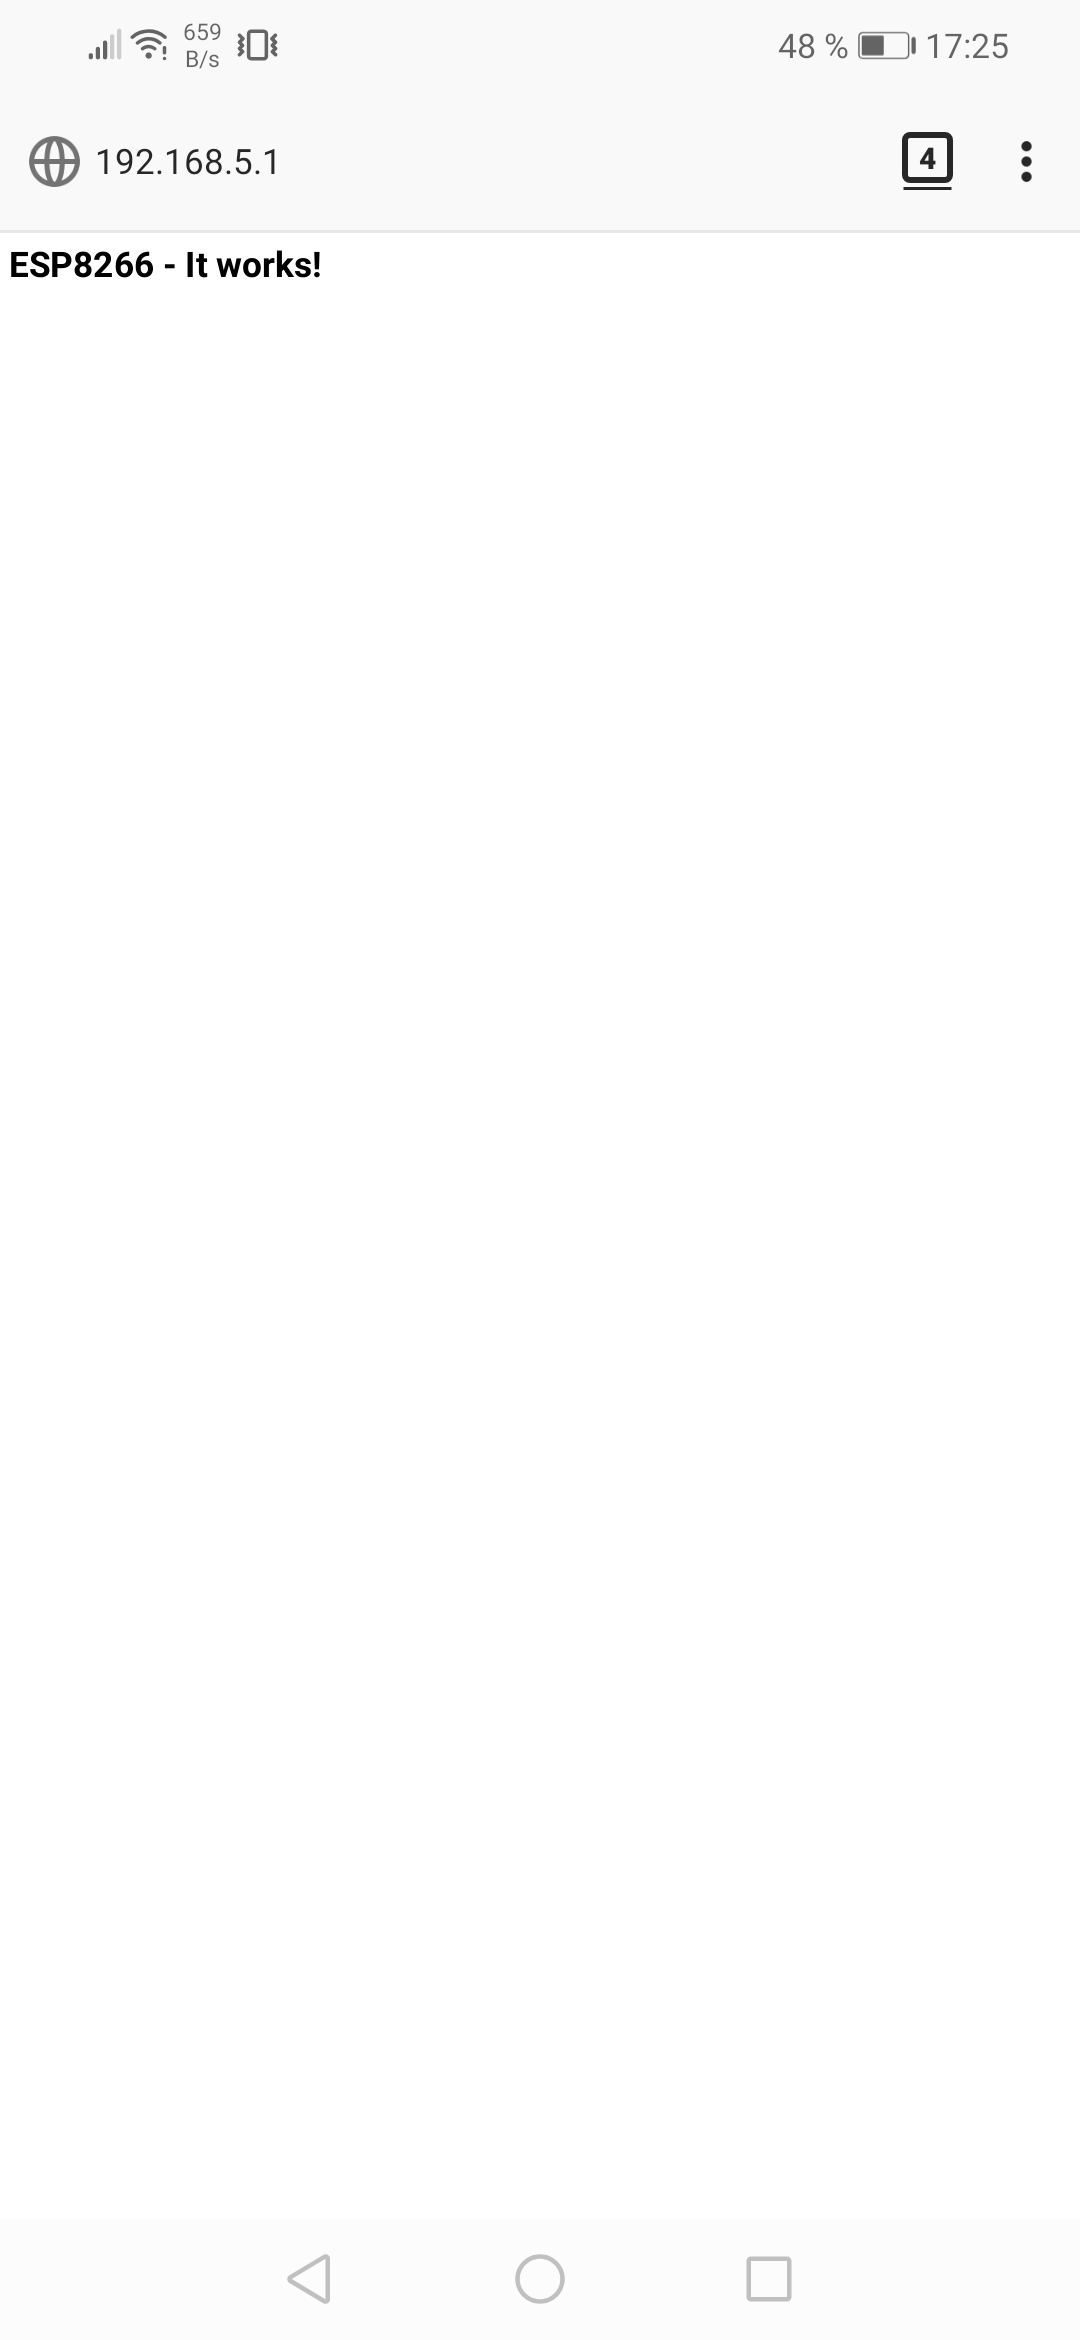
\includegraphics[scale=0.250]{image/11.jpg}
\caption{Site Web}
\label{fig:net }
\end{figure}
\begin{figure}[h!]
\centering
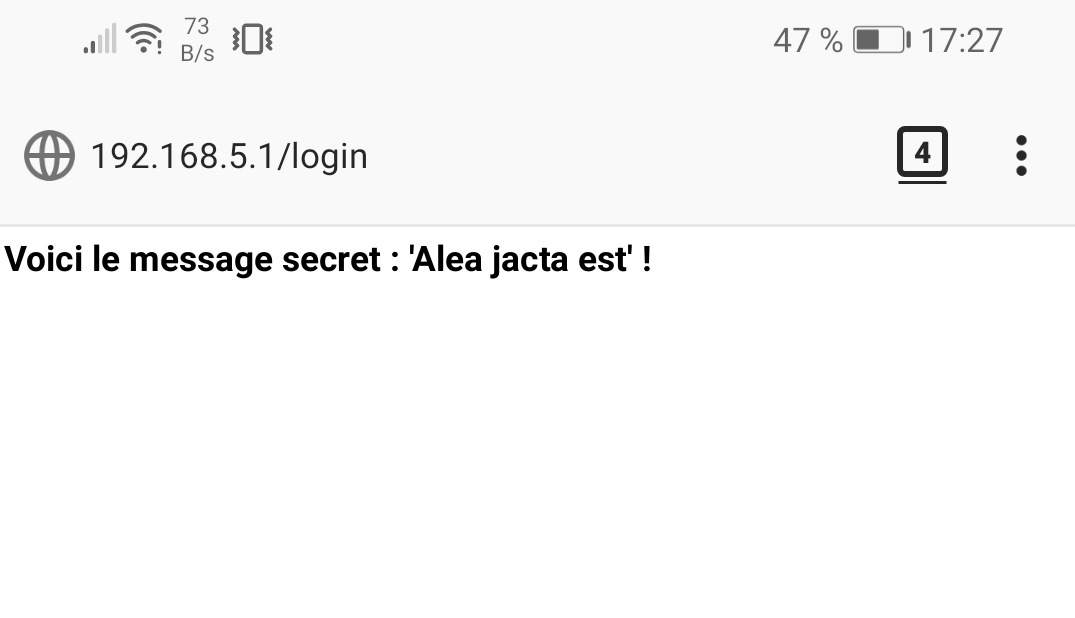
\includegraphics[scale=0.250]{image/10.jpg}
\caption{Site Web sécurisé}
\label{fig:net }
\end{figure}\\
\newpage
\section{Manipulation sur un site HTTPS}
On récuperé la capture de trame, et nous utilisons Aircrack pour déterminer la clé Wifi
\insertcode{https/aircrack}{Clé wifi}
Le Pass Wifi est donc: 53027819
On configure Wireshark pour qu'il comprenne les trames, puis avec le Pre-Master-Secret


\end{document}

